\documentclass{ximera}
\graphicspath{  %% When looking for images,
{./}            %% look here first,
{./pictures/}   %% then look for a pictures folder,
{../pictures/}  %% which may be a directory up.
{../../pictures/}  %% which may be a directory up.
{../../../pictures/}  %% which may be a directory up.
{../../../../pictures/}  %% which may be a directory up.
}

\usepackage{listings}
%\usepackage{circuitikz}
\usepackage{xcolor}
\usepackage{amsmath,amsthm}
\usepackage{subcaption}
\usepackage{graphicx}
\usepackage{tikz}
%\usepackage{tikz-3dplot}
\usepackage{amsfonts}
%\usepackage{mdframed} % For framing content
%\usepackage{tikz-cd}

  \renewcommand{\vector}[1]{\left\langle #1\right\rangle}
  \newcommand{\arrowvec}[1]{{\overset{\rightharpoonup}{#1}}}
  \newcommand{\ro}{\texttt{R}}%% row operation
  \newcommand{\dotp}{\bullet}%% dot product
  \renewcommand{\l}{\ell}
  \let\defaultAnswerFormat\answerFormatBoxed
  \usetikzlibrary{calc,bending}
  \tikzset{>=stealth}
  




%make a maroon color
\definecolor{maroon}{RGB}{128,0,0}
%make a dark blue color
\definecolor{darkblue}{RGB}{0,0,139}
%define the color fourier0 to be the maroon color
\definecolor{fourier0}{RGB}{128,0,0}
%define the color fourier1 to be the dark blue color
\definecolor{fourier1}{RGB}{0,0,139}
%define the color fourier 1t to be the light blue color
\definecolor{fourier1t}{RGB}{173,216,230}
%define the color fourier2 to be the dark green color
\definecolor{fourier2}{RGB}{0,100,0}
%define teh color fourier2t to be the light green color
\definecolor{fourier2t}{RGB}{144,238,144}
%define the color fourier3 to be the dark purple color
\definecolor{fourier3}{RGB}{128,0,128}
%define the color fourier3t to be the light purple color
\definecolor{fourier3t}{RGB}{221,160,221}
%define the color fourier0t to be the red color
\definecolor{fourier0t}{RGB}{255,0,0}
%define the color fourier4 to be the orange color
\definecolor{fourier4}{RGB}{255,165,0}
%define the color fourier4t to be the darker orange color
\definecolor{fourier4t}{RGB}{255,215,0}
%define the color fourier5 to be the yellow color
\definecolor{fourier5}{RGB}{255,255,0}
%define the color fourier5t to be the darker yellow color
\definecolor{fourier5t}{RGB}{255,255,100}
%define the color fourier6 to be the green color
\definecolor{fourier6}{RGB}{0,128,0}
%define the color fourier6t to be the darker green color
\definecolor{fourier6t}{RGB}{0,255,0}

%New commands for this doc for errors in copying
\newcommand{\eigenvar}{\lambda}
%\newcommand{\vect}[1]{\mathbf{#1}}
\renewcommand{\th}{^{\text{th}}}
\newcommand{\st}{^{\text{st}}}
\newcommand{\nd}{^{\text{nd}}}
\newcommand{\rd}{^{\text{rd}}}
\newcommand{\paren}[1]{\left(#1\right)}
\newcommand{\abs}[1]{\left|#1\right|}
\newcommand{\R}{\mathbb{R}}
\newcommand{\C}{\mathbb{C}}
\newcommand{\Hilb}{\mathbb{H}}
\newcommand{\qq}[1]{\text{#1}}
\newcommand{\Z}{\mathbb{Z}}
\newcommand{\N}{\mathbb{N}}
\newcommand{\q}[1]{\text{``#1''}}
%\newcommand{\mat}[1]{\begin{bmatrix}#1\end{bmatrix}}
\newcommand{\rref}{\text{reduced row echelon form}}
\newcommand{\ef}{\text{echelon form}}
\newcommand{\ohm}{\Omega}
\newcommand{\volt}{\text{V}}
\newcommand{\amp}{\text{A}}
\newcommand{\Seq}{\textbf{Seq}}
\newcommand{\Poly}{\textbf{P}}
\renewcommand{\quad}{\text{    }}
\newcommand{\roweq}{\simeq}
\newcommand{\rowop}{\simeq}
\newcommand{\rowswap}{\leftrightarrow}
\newcommand{\Mat}{\textbf{M}}
\newcommand{\Func}{\textbf{Func}}
\newcommand{\Hw}{\textbf{Hamming weight}}
\newcommand{\Hd}{\textbf{Hamming distance}}
\newcommand{\rank}{\text{rank}}
\newcommand{\longvect}[1]{\overrightarrow{#1}}
% Define the circled command
\newcommand{\circled}[1]{%
  \tikz[baseline=(char.base)]{
    \node[shape=circle,draw,inner sep=2pt,red,fill=red!20,text=black] (char) {#1};}%
}

% Define custom command \strikeh that just puts red text on the 2nd argument
\newcommand{\strikeh}[2]{\textcolor{red}{#2}}

% Define custom command \strikev that just puts red text on the 2nd argument
\newcommand{\strikev}[2]{\textcolor{red}{#2}}

%more new commands for this doc for errors in copying
\newcommand{\SI}{\text{SI}}
\newcommand{\kg}{\text{kg}}
\newcommand{\m}{\text{m}}
\newcommand{\s}{\text{s}}
\newcommand{\norm}[1]{\left\|#1\right\|}
\newcommand{\col}{\text{col}}
\newcommand{\sspan}{\text{span}}
\newcommand{\proj}{\text{proj}}
\newcommand{\set}[1]{\left\{#1\right\}}
\newcommand{\degC}{^\circ\text{C}}
\newcommand{\centroid}[1]{\overline{#1}}
\newcommand{\dotprod}{\boldsymbol{\cdot}}
%\newcommand{\coord}[1]{\begin{bmatrix}#1\end{bmatrix}}
\newcommand{\iprod}[1]{\langle #1 \rangle}
\newcommand{\adjoint}{^{*}}
\newcommand{\conjugate}[1]{\overline{#1}}
\newcommand{\eigenvarA}{\lambda}
\newcommand{\eigenvarB}{\mu}
\newcommand{\orth}{\perp}
\newcommand{\bigbracket}[1]{\left[#1\right]}
\newcommand{\textiff}{\text{ if and only if }}
\newcommand{\adj}{\text{adj}}
\newcommand{\ijth}{\emph{ij}^\text{th}}
\newcommand{\minor}[2]{M_{#2}}
\newcommand{\cofactor}{\text{C}}
\newcommand{\shift}{\textbf{shift}}
\newcommand{\startmat}[1]{
  \left[\begin{array}{#1}
}
\newcommand{\stopmat}{\end{array}\right]}
%a command to give a name to explorations and hints and theorems
\newcommand{\name}[1]{\begin{centering}\textbf{#1}\end{centering}}
\newcommand{\vect}[1]{\vec{#1}}
\newcommand{\dfn}[1]{\textbf{#1}}
\newcommand{\transpose}{\mathsf{T}}
\newcommand{\mtlb}[2][black]{\texttt{\textcolor{#1}{#2}}}
\newcommand{\RR}{\mathbb{R}} % Real numbers
\newcommand{\id}{\text{id}}
\newcommand{\coord}[1]{\langle#1\rangle}
\newcommand{\RREF}{\text{RREF}}
\newcommand{\Null}{\text{Null}}
\newcommand{\Nullity}{\text{Nullity}}
\newcommand{\Rank}{\text{Rank}}
\newcommand{\Col}{\text{Col}}
\newcommand{\Ef}{\text{EF}}
\newcommand{\boxprod}[3]{\abs{(#1\times#2)\cdot#3}}

\author{Zack Reed}
%borrowed from anna davis
\title{Unit Vectors}
\begin{document}
\begin{abstract}

    In this learning activity, you will be 
\end{abstract}
\maketitle

\section*{Unit Vector in the Direction of a Given Vector}
Recall that a {\it unit} vector is a vector of length 1.  Given a non-zero vector $\vec{v}$, we can find a unit vector in the same direction by multiplying $\vec{v}$ by an appropriate scalar.  For example, if $\vec{v}=\begin{bmatrix}a\\b\end{bmatrix}$ and $\norm{\vec{v}}=3$, then a unit vector $\vec{u}$ in the same direction is given by $\vec{u}=\begin{bmatrix}a/3\\b/3\end{bmatrix}=\begin{bmatrix}a/\norm{\vec{v}}\\b/\norm{\vec{v}}\end{bmatrix}$.


 
\begin{center}
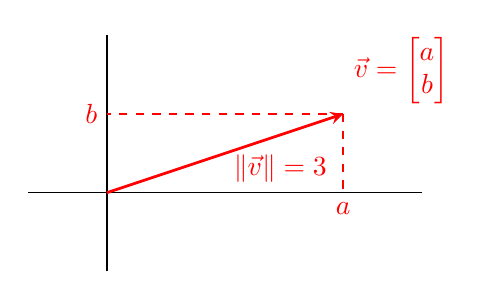
\begin{tikzpicture}


  \draw (-1,0)--(4,0);
  \draw (0,-1)--(0,2);



  \draw[line width=1pt,-stealth, red](0,0)--(3,1) node[above right]{$\vec{v}=\begin{bmatrix}a\\b\end{bmatrix}$};

  \draw[line width=0.5pt,dashed, red](3,1)--(3,0);
   \draw[line width=0.5pt,dashed, red](3,1)--(0,1);

    \node[red] at (3, -0.2)   (b) {$a$};
    \node[red] at (-0.2, 1)   (b) {$b$};
    \node[red] at (2.2, 0.3)   (b) {$\norm{\vec{v}}=3$};

\end{tikzpicture}
\end{center}


 
\begin{center}
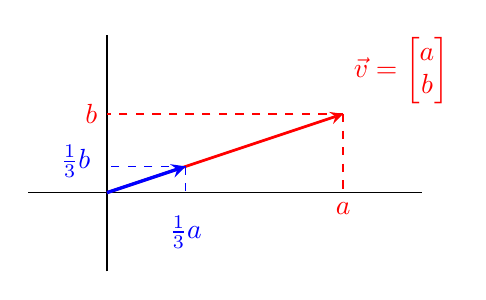
\begin{tikzpicture}
  \draw (-1,0)--(4,0);
  \draw (0,-1)--(0,2);
  \draw[line width=1pt,-stealth, red](0,0)--(3,1) node[above right]{$\vec{v}=\begin{bmatrix}a\\b\end{bmatrix}$};
  \draw[line width=0.5pt,dashed, red](3,1)--(3,0);
   \draw[line width=0.5pt,dashed, red](3,1)--(0,1);
\node[red] at (3, -0.2)   (b) {$a$};
    \node[red] at (-0.2, 1)   (b) {$b$};
    \draw[line width=1.2pt,-stealth, blue](0,0)--(1,1/3);
  \draw[line width=0.5pt,dashed, blue](1,1/3)--(1,0);
   \draw[line width=0.5pt,dashed, blue](1,1/3)--(0,1/3);
   \node[blue] at (1, -0.5)   (b) {$\frac{1}{3}a$};
    \node[blue] at (-0.4, 0.4)   (b) {$\frac{1}{3}b$};
  \end{tikzpicture}
\end{center}
 
In general, dividing a non-zero vector by its own magnitude produces a unit vector in the same direction.  We summarize this observation in a theorem.


 
 
  \begin{theorem}\label{th:unit} Let $\vec{v}=\begin{bmatrix}v_1\\v_2\\\vdots\\v_n\end{bmatrix}$ be a non-zero vector in $\mathbb{R}^n$. Vector $\vec{u}$ given by
  \begin{equation*}
 \vec{u}=\frac{1}{\norm{\vec{v}}}\vec{v}=\begin{bmatrix}v_1/\norm{\vec{v}}\\v_2/\norm{\vec{v}}\\\vdots\\v_n/\norm{\vec{v}}\end{bmatrix}
\end{equation*}
is a unit vector in the direction of $\vec{v}$.
\end{theorem}



 
\begin{proof}
Because $\vec{u}$ is a positive scalar multiple of $\vec{v}$, $\vec{u}$ points in the direction of $\vec{v}$.  We now show that $\norm{\vec{u}}=1$.
\begin{eqnarray*}
\norm{\vec{u}}&=&\sqrt{ \Big(\frac{v_1}{\norm{\vec{v}}}\Big)^2+\Big(\frac{v_2}{\norm{\vec{v}}}\Big)^2+\ldots +\Big(\frac{v_n}{\norm{\vec{v}}}\Big)^2}\\
&=&\frac{1}{\norm{\vec{v}}}\sqrt{v_1^2+v_2^2+\ldots +v_n^2}\\
&=&\frac{\norm{\vec{v}}}{\norm{\vec{v}}}=1
\end{eqnarray*}
\end{proof}
 

 
\begin{example}\label{reference}
Find a unit vector in the direction of $\vec{v}=\begin{bmatrix}2\\-3\\1\\0\\1\end{bmatrix}$.
 
\begin{explanation}
We first compute $\norm{\vec{v}}$.
$$\norm{\vec{v}}=\sqrt{4+9+1+1}=\sqrt{15}$$
By Theorem \ref{th:unit},
$$\vec{u}=\begin{bmatrix}2/\sqrt{15}\\-3/\sqrt{15}\\1/\sqrt{15}\\0\\1/\sqrt{15}\end{bmatrix}=\frac{1}{\sqrt{15}}\begin{bmatrix}2\\-3\\1\\0\\1\end{bmatrix}$$
\end{explanation}
\end{example}

 
\section*{Practice Problems}
\begin{problem}
    Find a unit vector in the direction of the given vector $\vec{v}$.
  \begin{problem}\label{prob:00361}
  $\vec{v}=\begin{bmatrix}-3\\4\end{bmatrix}$
 
  Answer: $\vec{u}=\begin{bmatrix}\answer{-0.6}\\\answer{0.8}\end{bmatrix}$
  \end{problem}
  \begin{problem}\label{prob:00362}
      $\vec{v}=\begin{bmatrix}2\\-3\\6\end{bmatrix}$
 
Answer:$\vec{u}=\begin{bmatrix}\answer{2/7}\\\answer{-3/7}\\\answer{6/7}\end{bmatrix}$
   \end{problem}
   \begin{problem}\label{prob:00363}
        $\vec{v}=\begin{bmatrix}1\\3\\-2\end{bmatrix}$
 
 Answer: $\vec{u}=\begin{bmatrix}\answer{1/\sqrt{14}}\\\answer{3/\sqrt{14}}\\\answer{-2/\sqrt{14}}\end{bmatrix}$      
  \end{problem}
\end{problem} 
\begin{problem}\label{prob:00364}
Let $\vec{v}=\begin{bmatrix}-1\\1\\\sqrt{7}\end{bmatrix}$.
Apply the concepts from this section to find a vector $\vec{w}$ that points in the same direction as $\vec{v}$ and whose length is 5.
 
Answer: $\vec{w}=\begin{bmatrix}
    \answer{-5/3}\\\answer{5/3}\\\answer{5\sqrt{7}/3}
\end{bmatrix}$
\end{problem}


\end{document}